% HEADER
\documentclass[class=article, crop=false]{standalone}
\usepackage{00_Preamble/frr_preamble}

% Packages
\usepackage{titlesec}
\usepackage{hyperref}
\usepackage{float}
\usepackage{graphics}
\usepackage{placeins}
\usepackage{adjustbox}
% END HEADER

\begin{document}
	\subsection{Final Design}
	\label{subsec:final-design}
	
	After the preliminary design was completed, several design iterations were made as the CAD assembly was further developed and specific parts were selected. Changes were made to resolve size constraint issues, reduce fabrication time, and reduce system cost. The final CAD assembly of the robot is presented in Figure \ref{fig:final-cad}.
	
	\FloatBarrier
	\begin{figure}[h]
	\centering
	 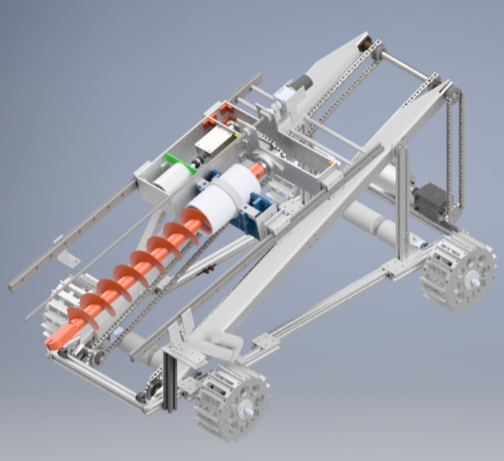
\includegraphics[width=0.5\linewidth]{09_Figures/final-cad.jpg}
	 \caption{Final Robot CAD Assembly}
	 \label{fig:final-cad}
	\end{figure}
	\FloatBarrier
	
	\subsubsection{Frame Section}
	
<<<<<<< HEAD
	The frame was designed to be lightweight and simple to modify (Figure \ref{fig:frame-cad}). It was constructed from 30mm by 30mm aluminum extrusions connected by corner brackets and flat mounting plates. Two vertical supports near the back connect the conveyor. The motor and gearbox that drive the conveyor were placed on the back extrusion. Only minor length changes were made to the frame between the preliminary design review and the final design. The final weight was under 4 kg.
=======
	The frame was designed to be lightweight and simple to modify (Fig. 7). It was constructed from 30mm by 30mm aluminum extrusions connected by corner brackets and flat mounting plates. Two vertical supports near the back connect the conveyor. The motor and gearbox that drive the conveyor were placed on the back extrusion. Only minor length changes were made to the frame between the preliminary design review and the final design. The final weight, excluding the wheels, was under 4 kg.
>>>>>>> 78a240ce2f48d44d712c7fba2ab129acb4495ae5
	
	The wheel diameter was reduced to 7.875 inches since the rover was above the RMC height limit with the previous 30 cm diameter. The units were switched from metric to U.S. customary to aid in machining. The motor mount height was also decreased to lower the robot height.

	The final wheel design (Figure \ref{fig:wheel-cad}) was modified to be easier to fabricate. The first design had a lot of components that would make assembly challenging and could lead to points of failure. The wheel rim was eliminated to decrease weight. It did not provide much structural support, as most of the load is distributed through the sides of the wheel. The grousers are press fit and bolted into the wheel sides instead of using 3D printed spacers. The number of grousers was increased from twelve to eighteen. This increases traction and smoothes the ride. 

	VEX CIM motors were chosen to drive the wheels. The motors provide a maximum of 337 Watts. VEX parts are easy to assemble, as all the parts interface well together. Hex shafts were used over rotary shafts to increase the torque transmission between the axles and the wheels.
	
	
	\begin{figure}
	\centering
	\begin{minipage}{.5\textwidth}
	  \centering
	  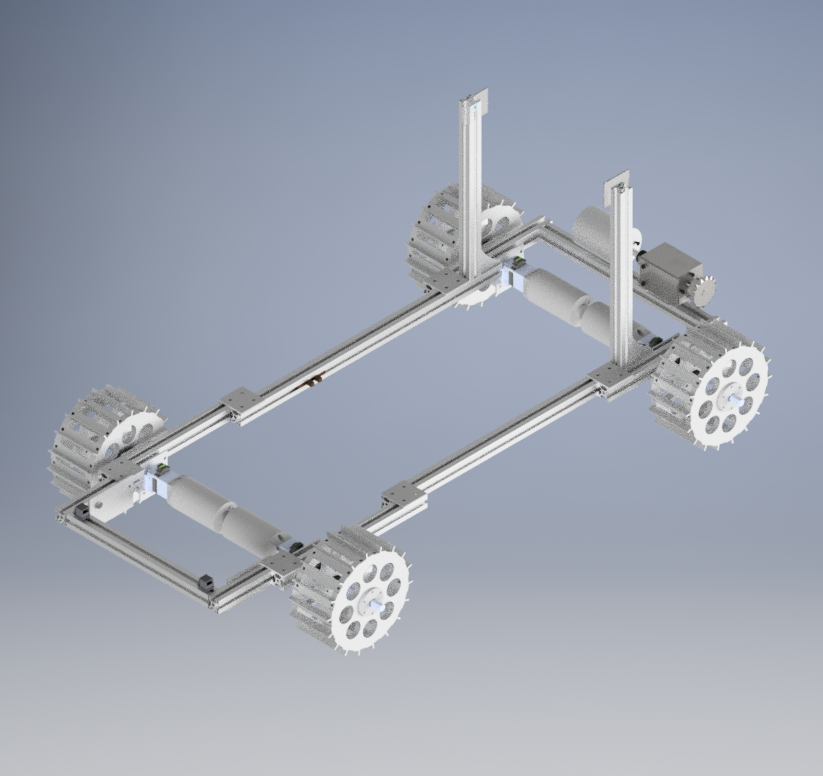
\includegraphics[width=.4\linewidth]{09_Figures/frame-cad.jpg}
	  \captionof{figure}{Final CAD Frame Assembly}
	  \label{fig:frame-cad}
	\end{minipage}
	\begin{minipage}{.5\textwidth}
	  \centering
	  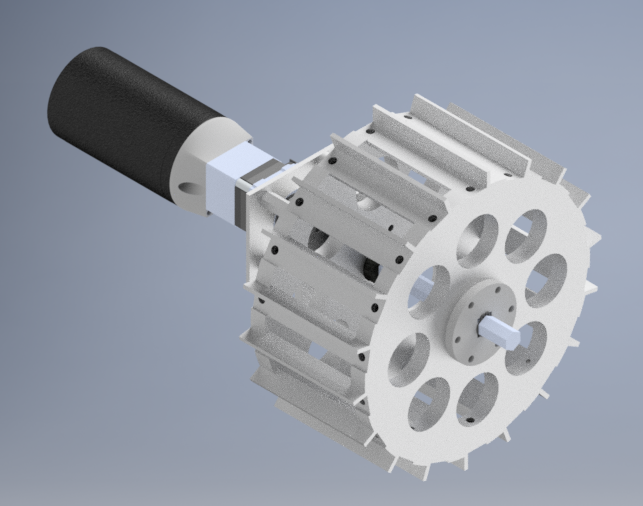
\includegraphics[width=.4\linewidth]{09_Figures/wheel-cad.jpg}
	  \captionof{figure}{Final Wheel Assembly}
	  \label{fig:wheel-cad}
	\end{minipage}
	\end{figure}
	
	
%	\begin{wrapfigure}{l}{0.4\textwidth}
%	\centering
%	 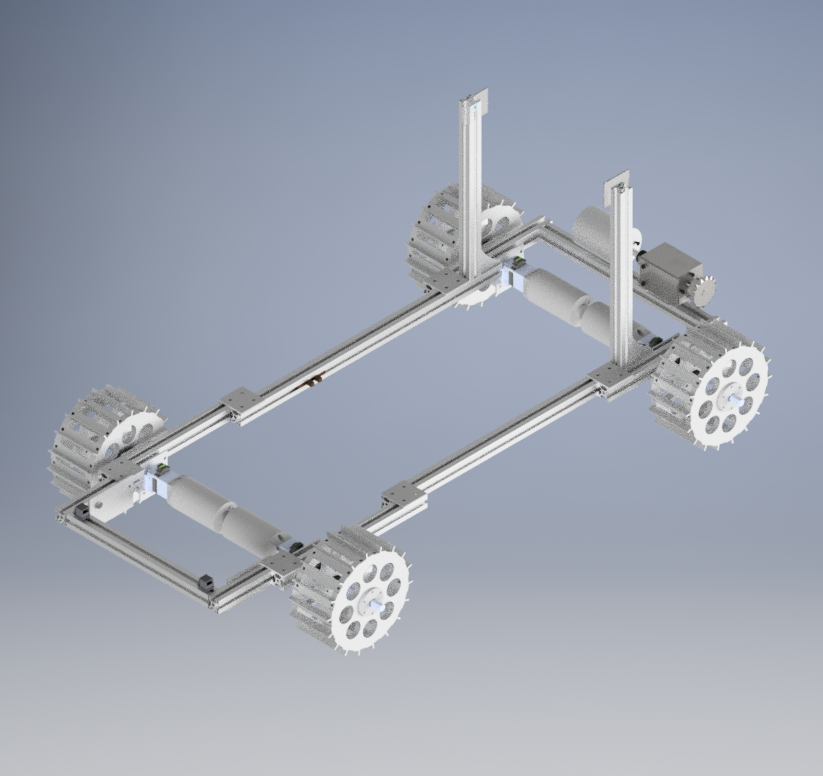
\includegraphics[width=0.4\linewidth]{09_Figures/frame-cad.jpg}
%	 \caption{Final CAD Frame Assembly}
%	 \label{fig:frame-cad}
%	\end{wrapfigure}
%	
%	\begin{wrapfigure}{r}{0.4\textwidth}
%	\centering
%	 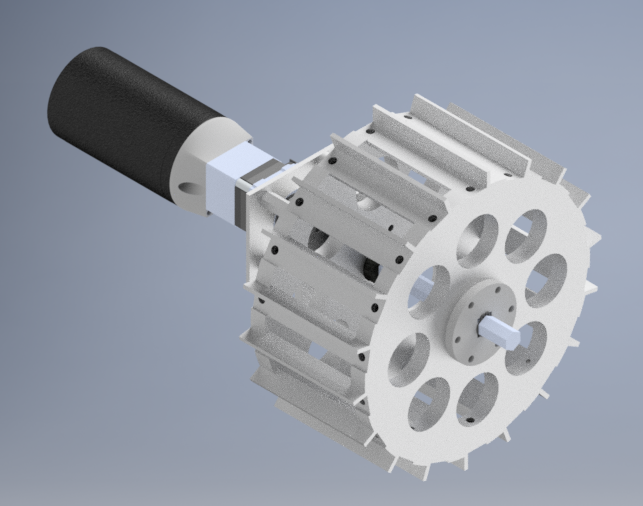
\includegraphics[width=0.4\textwidth]{09_Figures/wheel-cad.jpg}
%	 \caption{Final }
%	 \label{fig:wheel-cad}
%	\end{wrapfigure}
	
	
	
	\subsubsection{Cost Budget}
	
	\subsubsection{Management Structure}
	Team members were distributed among three subgroups, mechanical, electrical, and programming, based on their area of interest and expertise. Members of each subteam were assigned to specific subsystems of the robot and worked in cross-disciplinary groups with other members from each subteam to fully design the subsystem. The purpose of the cross-functional groups was to ensure that all aspects of the design are considered simultaneously. Each of the subteams were managed by a subteam lead, whose responsibility was to allocate work and track progress for the design of their respective part of the robot. The subteam leads reported their progress to the team captain. The captain was responsible for tracking objectives, facilitating integration between various subteams, and ensuring that the high-level requirements are met.



	
	
	


	
\end{document}
